% chktex-file 8 36 26 38 32
\documentclass[a4paper,12pt]{article}

% Packages
\usepackage[utf8]{inputenc}
\usepackage{graphicx}
\usepackage{hyperref}
\usepackage{geometry}
\geometry{margin=1in}
\usepackage{titlesec}
\usepackage{fancyhdr}
\usepackage{listings}
\usepackage{longtable}
\usepackage{booktabs}
\usepackage{xcolor}
\usepackage{minted}
\usepackage{colortbl}
\usepackage{setspace}
\usepackage[utf8]{inputenc}
\usepackage{newunicodechar}
\usepackage{amssymb}
\usepackage{lmodern} 
\usepackage{silence}
\WarningFilter{fancyhdr}{\headheight is too small}

\newunicodechar{✓}{\checkmark}  
\usepackage[most]{tcolorbox}
\tcbuselibrary{minted, listingsutf8}
\setminted{breaklines}

\newtcblisting{code}[2][]{%
  listing engine=minted,
  colback=white,
  colframe=black,
  listing only,
  minted language=#2,
  minted options={fontsize=\small, linenos, breaklines,
                  breaksymbolleft=, breaksymbolright=, #1},
  sharp corners,
  boxrule=0.8pt,
  left=5pt,
  right=5pt,
  top=8pt,
  bottom=8pt,
  enhanced,
  breakable
}


% Customize listings appearance

\lstset{
  basicstyle=\ttfamily\small,
  keywordstyle=\color{blue},
  stringstyle=\color{red},
  commentstyle=\color{green!50!black},
  breaklines=true,
  frame=single,
  numbers=left,
  numberstyle=\tiny,
  stepnumber=1,
  numbersep=5pt,
  showstringspaces=false,
  tabsize=2,
}

% Header and footer setup for all pages except cover
\fancypagestyle{main}{
  \fancyhf{}
  \rhead{CSC381 - E-Commerce}
  \lhead{Lab 2: Introduction for JavaScript}
  \cfoot{\thepage}
  \renewcommand{\headrulewidth}{0.4pt}
  \renewcommand{\footrulewidth}{0.4pt}
}

\title{Lab Report 2: Introduction for JavaScript to E-commerce}
\author{Submitted by: Parakram Kharel \\ Roll No: 24 \\ 
\textit{Kathford International College of Engineering and Management} \\ 
Affiliated to Tribhuvan University}
% \date{\today}
\makeatletter
\begin{document}
% \date{August 17, 2025}

% --------- Cover Page ---------
\begin{titlepage}
  \begin{center}
    \vspace*{2cm}
    
\includegraphics[width=0.35\textwidth]{Kath.png} \\[2cm]

    {\Huge \bfseries Lab Report 2} \\[0.5cm]
    {\Large Introduction for JavaScript to E-commerce} \\[2cm]

    {\Large \textbf{Course:} CSC381 - E-Commerce} \\[1cm]
    {\Large \textbf{Submitted by:}} \\[0.3cm]
    {\large Parakram Kharel \\ Roll No: 24} \\[2cm]

    \textit{Kathford International College of Engineering and Management} \\
    Affiliated to Tribhuvan University \\[3cm]
    
    \date{August 23, 2025}
    {\normalsize \@date}
    % \today
  \end{center}
\end{titlepage}

% Use fancy header/footer for the rest of the document
\pagestyle{main}
\setlength{\parskip}{1em}

% --------- Content ---------
\section*{1. Objective}
To implement product price display, simple calculations, and interactive UI elements for an e-commerce web application using JavaScript, building upon the HTML/CSS foundation created in Lab 1.


\section*{2. Tools and Technologies Used}
\begin{longtable}{ll}
\toprule
\textbf{Technology} & \textbf{Purpose} \\
\midrule
HTML5 & Structure and semantic markup for product displays \\
CSS3 & Styling, animations, and responsive design \\
JavaScript & Price calculations and interactive functionality \\
VS Code & Code editor and development environment \\
Web Browser Developer Tools & Debugging and performance testing \\
\bottomrule
\end{longtable}

\section*{3. Theory / Background}
JavaScript is a powerful scripting language that is used to create dynamic and interactive content on Web pages. Unlike HTML and CSS, which define structure and style, JavaScript enables real-time functionality such as responding to user actions, updating content without reloading the page, and performing calculations in the browser.

In this lab, JavaScript is used to enhance the product catalog by implementing interactive features such as quantity selectors, price formatting, discount calculations, and responsive UI behavior. These dynamic elements improve the overall user experience and bring essential e-Commerce functionality to the web interface.

\section*{4. Page Layout Design}
\subsection*{4.1 Product Card Structure}
Each interactive product card now contains the following: 
\begin{itemize}
  \item Product Image with dynamic badges (NEW, SALE, HOT)
  \item Product Title and Description
  \item Enhanced Price Section with:
    \begin{itemize}
      \item Current price display with proper formatting
      \item Original price with strike through for sale items
      \item Automatic discount percentage calculation
      \item Savings amount display
    \end{itemize}
  \item Interactive Quantity Section featuring:
    \begin{itemize}
      \item Increment/decrement buttons with validation
      \item Number input field (1--10 range)
      \item Real-time total calculation display
    \end{itemize}
  \item Action buttons with visual feedback
\end{itemize}

\subsection*{4.2 Interactive Features Implementation}
\begin{itemize}
  \item Real-time price calculations based on quantity selection
  \item Dynamic discount percentage and savings computations
  \item Visual feedback animations for button interactions
  \item Responsive quantity selectors with input validation
  \item Enhanced search functionality including price-based filtering
  \item Category filtering with smooth transition effects
\end{itemize}

\subsection*{4.3 JavaScript Functionality Components}
\begin{itemize}
  \item Price formatting functions for proper currency display
  \item Mathematical calculation functions for discounts, taxes, and shipping
  \item Event listeners for user interactions and input validation
  \item DOM manipulation for dynamic content updates
  \item Animation control through programmatic CSS class manipulation
\end{itemize}

\section*{5. Code Snippets}

\subsection*{5.1 HTML Code: Product Card with Interactive Elements}
% chktex-file 8
\begin{code}[fontsize=\small]{html}
<div class='product-card' data-category='electronics'>
    <div class='product-image'>
        <img src='images/headphone.jpg' alt='Wireless Headphones'>
        <div class='product-badge'>NEW</div>
    </div>
    <div class='product-info'>
        <h3>Premium Headphones</h3>
        <p class='product-desc'>
            High-quality wireless headphones with noise cancellation
        </p>
        <div class='price-section'>
            <div class='price-tag' data-original-price='8999'>NPR 8,999</div>
            <div class='discount-info' style='display: none;'>
                <span class='discount-percent'></span>
                <span class='savings-amount'></span>
            </div>
        </div>
        <div class='quantity-section'>
            <label>Quantity:</label>
            <div class='quantity-selector'>
                <button class='qty-btn minus' onclick='changeQuantity(this, -1)'> - </button>
                <input type='number' class='qty-input' value='1' min='1' max='10' onchange='updateProductTotal(this)'>
                <button class='qty-btn plus' onclick='changeQuantity(this, 1)'>+</button>
            </div>
            <div class='product-total'>
                Total: NPR <span class='total-amount'>8,999</span>
            </div>
        </div>
        <div class='product-actions'>
            <button class='select-btn' data-price='8999'>Select Item</button>
            <button class='details-btn'>View Details</button>
        </div>
    </div>
</div>
\end{code}

\subsection*{5.2 JavaScript Code: Price Formatting Functions}
\begin{code}[fontsize=\small]{javascript}
function formatPrice (price) {
    return price.toLocaleString('en-NP');
}

function formatCurrency (amount) {
    return `NPR ${formatPrice(amount)}`;
}
\end{code}

\subsection*{5.3 JavaScript Code: Discount Calculation}
\begin{code}[fontsize=\small]{javascript}
function calculateDiscount(originalPrice, salePrice) {
    const discount = originalPrice - salePrice;
    const discountPercent = Math.round((discount / originalPrice) * 100);
    return {
        percent: discountPercent,
        amount: discount,
        savings: formatCurrency(discount)
    };
}
\end{code}

\subsection*{5.4 JavaScript Code: Quantity Management}
\begin{code}[fontsize=\small]{javascript}
function changeQuantity(button, change) {
    const qtyInput = button.parentNode.querySelector('.qty-input');
    const currentValue = parseInt(qtyInput.value);
    const newValue = currentValue + change;

    if (newValue >= 1 && newValue <= 10) {
        qtyInput.value = newValue;
        updateProductTotal(qtyInput);
    }
}

function updateProductTotal(input) {
    const quantity = parseInt(input.value);
    const productCard = input.closest('.product-card');
    const priceTag = productCard.querySelector('.price-tag');
    const originalPrice = parseInt(priceTag.getAttribute('data-original-price'));

    const totalAmount = originalPrice * quantity;
    const totalAmountElement = productCard.querySelector('.total-amount');
    totalAmountElement.textContent = formatPrice(totalAmount);
}
\end{code}

\subsection*{5.5 JavaScript Code: Interactive UI Elements}
\begin{code}[fontsize=\small]{javascript}
function selectItem(productName, quantity, button) {
    selectedItemsCount++;
    updateItemsDisplay();
    showButtonFeedback(button);

    const quantityText = quantity > 1 ? ` (x${quantity})` : '';
    showNotification(`${productName}${quantityText} selected!`);
}

function showButtonFeedback(button) {
    const originalText = button.textContent;
    button.textContent = '✓ Selected!';
    button.style.background = 'linear-gradient(135deg, #48bb78, #38a169)';
    
    setTimeout(() => {
        button.textContent = originalText;
        button.style.background = 'linear-gradient(135deg, #667eea, #764ba2)';
    }, 1500);
}

\end{code}


\section*{6. Output / Screenshots}
\begin{center}
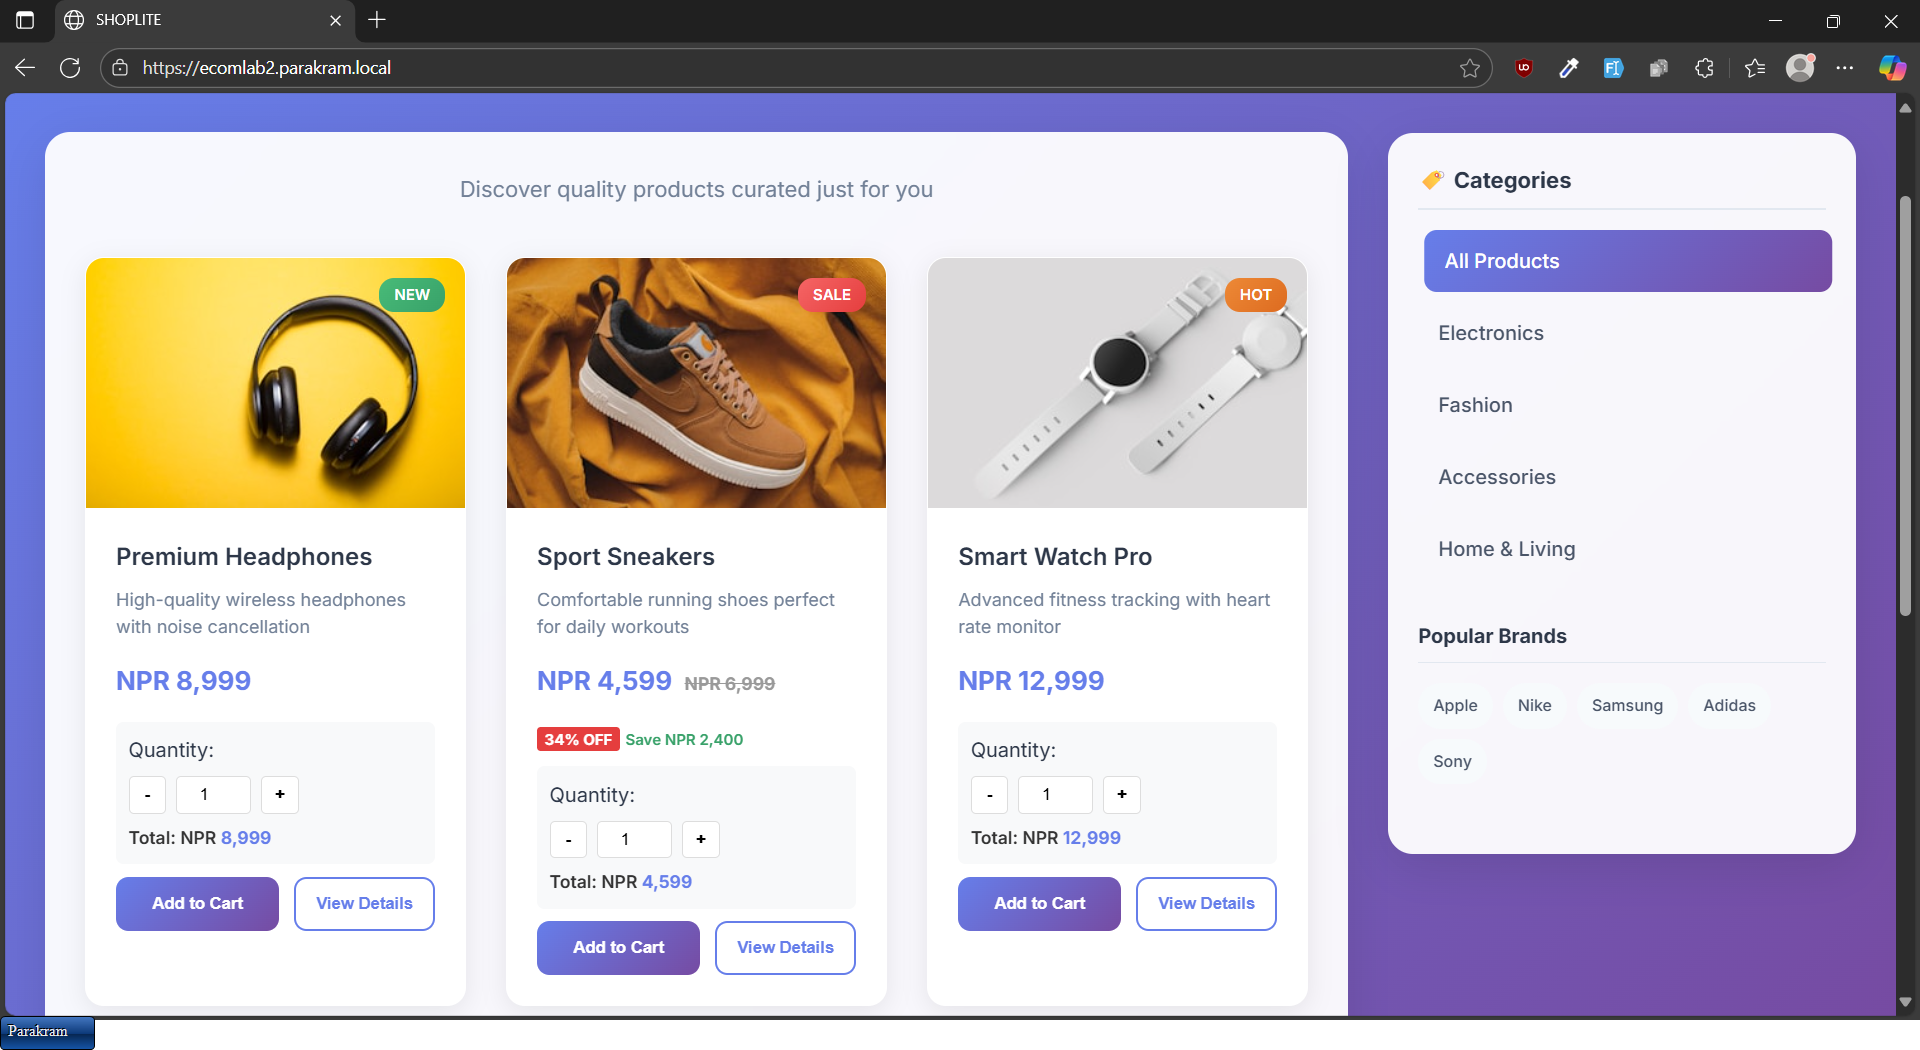
\includegraphics[width=\textwidth,height=8cm,keepaspectratio]{images/output1.png} 
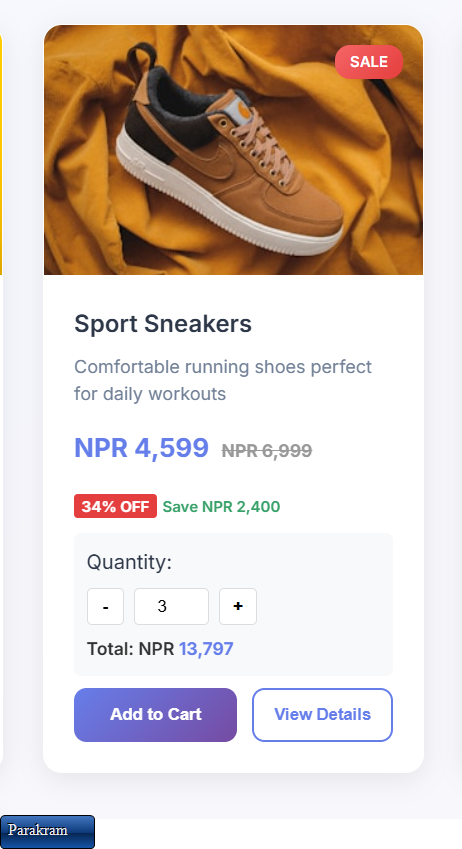
\includegraphics[width=0.7\textwidth, height=7cm, keepaspectratio]{images/output2.png}
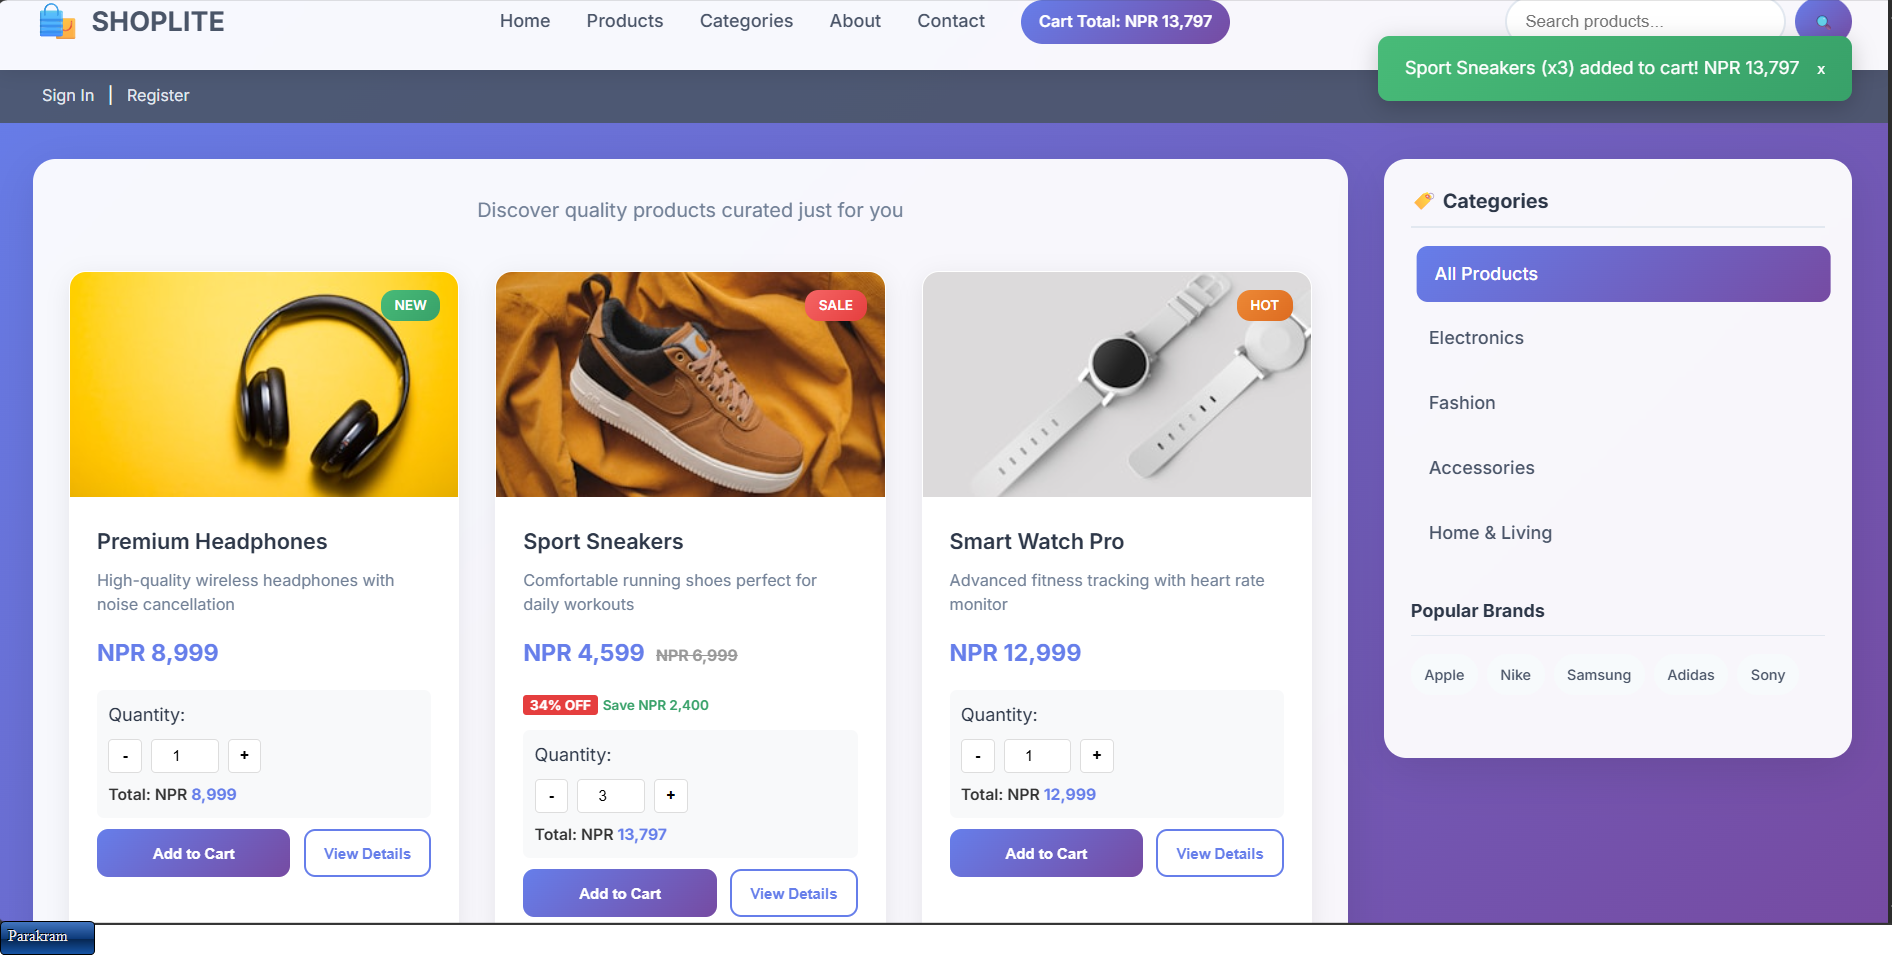
\includegraphics[width=\textwidth,height=8cm,keepaspectratio]{images/output3.png} 

\end{center}

\section*{7. Result}
The enhanced product catalog features dynamic JavaScript, including real-time price calculations, interactive quantity selectors, automatic discounts, and instant total updates. Prices are in NPR, and visual feedback like animations and color changes improves the user experience. Users can adjust quantities, see totals instantly, receive selection notifications, and filter searches by price.

\section*{8. Conclusion}
This lab demonstrated how JavaScript integrates with HTML and CSS to build dynamic e-commerce features. Students learned to format prices, create interactive UI components with event handling, and perform real-time calculations for pricing and discounts. It provided a strong foundation in DOM manipulation, event-driven programming, and data validation, showing how static HTML can become responsive, user-driven interfaces.

\section*{9. References}
\begin{itemize}
  \item \href{https://developer.mozilla.org/en-US/docs/Web/JavaScript}{MDN JavaScript Documentation}
  \item \href{https://javascript.info/}{The Modern JavaScript Tutorial}
  \item \href{https://www.w3schools.com/js/}{W3Schools JavaScript Tutorial}
  \item \href{https://developer.mozilla.org/en-US/docs/Web/JavaScript/Reference/Global_Objects/Intl/NumberFormat}{MDN NumberFormat API Documentation}
\end{itemize}
\end{document}

